\newcommand{\basedir}{fablab-document}
\documentclass{\basedir/fablab-document}

\usepackage{minitoc} % Inhaltsübersicht je Section
% \usepackage{fancybox} %ovale Boxen für Knöpfe - nicht mehr benötigt
\usepackage{amssymb} % Symbole für Knöpfe
% \usepackage{subfigure,caption}
\usepackage{eurosym}
\usepackage{tabularx} % Tabellen mit bestimmtem Breitenverhältnis der Spalten
\usepackage{wrapfig} % Textumlauf um Bilder
\usepackage{todonotes}

\renewcommand{\texteuro}{\euro}

\linespread{1.2}

\date{März 2016}
\author{Philipp Hörauf (Überarbeitung C. Kotzott)}
\title{Einweisung Oberfräse}

\begin{document}
 % Hinweise an Package minitoc, doch bitte irgendwas zu generieren - wird für späteres \secttoc benötigt
\dosecttoc
\faketableofcontents
\mtcsettitle{secttoc}{Arbeitsschritte}
\mtcsettitlefont{secttoc}{\large \sffamily \bfseries}
\mtcsetfont{secttoc}{subsection}{\sffamily}
% \mtcset
% hier geht das eigentliche Dokument los

\color{red}
\hrule
\begin{center}
\large{Achtung! Einweisung ist noch in Arbeit!}
\vspace{0.1cm}
\end{center}
\hrule
\color{black}

\section[Allgemeine Sicherheitshinweise]{Allgemeine Sicherheitshinweise}
\begin{itemize}
\item Hände bei aktiver Oberfräse immer vom Fräsbereich und dem Fräser fernhalten.
\item Die Oberfräse immer mit beiden Händen halten, entweder an Drehknopf, Handgriff und/oder den elektrisch isolierten Teilen des Gehäuses. Wenn beide Hände die Oberfräse halten, können sie vom Fräser nicht verletzt werden.
\item Nicht unter das Werkstück greifen.
\item Die Frästiefe an die Dicke des Werkstückes anpassen.
\item Netzkabel aus dem Eingriffsbereich des Fräsers halten. Die Metallteile des Elektrowerkzeugs könnten sonst unter Spannung stehen und einen elektrischen Schlag verursachen.
\item Das zu fräsende Werkstück niemals in der Hand, über dem Bein halten oder von Dritten halten lassen. Das Werkstück stabil und sicher fixieren. Es ist wichtig, das Werkstück gut zu befestigen, um die Gefahr bei Körperkontakt, Klemmen des Fräsers oder Verlust der Kontrolle zu minimieren.
\item Werkzeug fest einspannen - dazu Schlüssel aus der Maschinenkiste verwenden
\item Nur Fräser der richtigen Größe verwenden. Fräser, die nicht zur Maschine passen, können zu Verlust der Kontrolle, schweren Verletzungen oder Beschädigung der Maschine führen.
\item Immer mit Absaugung fräsen.
\item Nur im Gegenlauf fräsen. (siehe Abb. 7)
\item Korrekte Drehzahl für jeweiliges Werkzeug und Werkstück vorwählen (siehe Abb. 1)
\item Niemals beschädigte Fräser verwenden. Es besteht die Gefahr des Festfressens oder Abreißens des Fräsers. Als beschädigt gelten Fräser dann, wenn sie Risse, Ausbrüche oder Verformungen zeigen oder schlichtweg abgenutzt und stumpf sind.
\item Vor Werkzeugwechsel Maschine vom Stromnetz trennen, z.B. Stecker ziehen.
\item Nach dem Fräsen von Aluminium Maschine gründlichst reinigen und aussaugen.
\item Beim Fräsen immer einen Anschlag oder eine Führung verwenden. Dies verbessert die Genauigkeit und verringert die Gefahr, dass der Fräser verklemmt/sich festfrisst. Führung oder Anschlag bestimmungsgemäß fixieren.
\item Im Arbeitsbereich dürfen sich keine Unbeteiligten befinden
\end{itemize}

\newpage

\section{Persönliche Schutzausrüstung}

\begin{itemize}
\item Gehörschutz
\item Schutzbrille bei Bearbeitung von Aluminium, Faserwerkstoffen und Gipskarton
\item Staubmaske bei stauberzeugenden Arbeiten (Stäube von Harthölzern gelten als gesundheitsschädlich!)
\item Schutzhandschuhe beim Bearbeiten rauher Materialien und beim Werkzeugwechsel.
\item Keine weite Kleidung, Schals, Kleidungsstücke mit langen Bändeln etc. tragen. Diese können in die Maschine gezogen werden!
\end{itemize}

\section{Bestimmungsgemäße Verwendung}
Die Oberfräse ist ein nützliches Gerät zur Bearbeitung von Kanten, zum Versäubern und auch zur kreativen Gestaltung (z.b. Einfräsen von Schrift oder Löchern in Plattenmaterial). Sie birgt, korrekt angewendet, nur ein geringes Verletzungsrisiko. Dennoch ist es wichtig, die folgenden Anweisungen genau zu beachten, damit die Oberfräse nicht zu Gesundheitsschäden führt oder beschädigt wird.\\

Oberfräsen sind bestimmungsgemäß zum Fräsen von Holz, Kunststoffen und holzähnlichen Werkstoffen vorgesehen. Mit dafür vorgesehenen Fräswerkzeugen kann auch Aluminium oder Gipskarton bearbeitet werden. Es dürfen nur Fräser mit folgenden Daten verwendet werden:

\begin{itemize}
\item Schaftdurchmesser 8mm (Spannzangen für Fräser mit 6 bzw. 6,35mm Durchmesser sind erhältlich aber nicht vorhanden.)
\item Fräserdurchmesser max. 35mm
\item Die maximal für den Fräser erlaubte Drehzahl darf nicht überschritten werden.
\end{itemize}

\begin{figure}[]
	\centering
	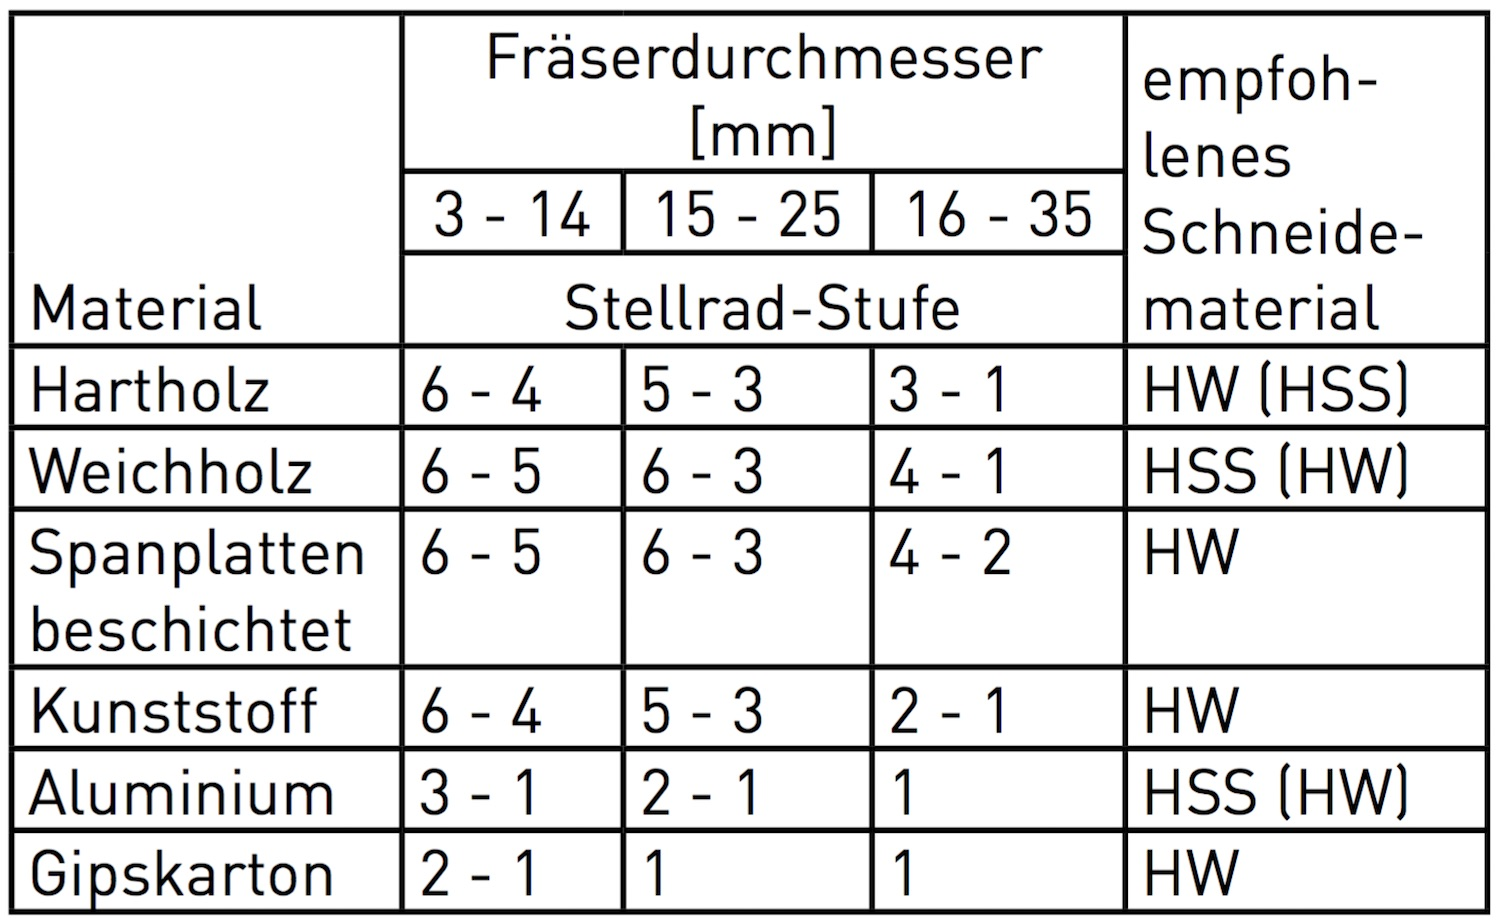
\includegraphics[width=0.6\textwidth]{img/schnittwerte.jpg}
	\caption{empfohlene Werkzeugdrehzahlen}
	\label{fig:werkzeugdrehzahl}
\end{figure}

Bei der Verwendung der Maschine muss \textbf{IMMER} der Festool-Staubsauger verwendet werden. Dabei ist zu beachten, dass die Oberfräse an der Steckdose 1 des Saugers angeschlossen wird und der Sauger auf \enquote{AUTO} steht. Sauger mindestens auf halbe Kraft, besser auf Vollgas stellen.\\

\textbf{WICHTIG: Die Oberfräse darf ausschließlich von eingewiesenen Personen verwendet werden.}


\subsection{Aluminiumbearbeitung}
Bei der Bearbeitung von Aluminium sind aus Sicherheitsgründen folgende besonderen Maßnahmen einzuhalten:
\begin{itemize}
\item Maschine an den Festool-Absaugwagen anschließen.
\item Maschine nach der Arbeit von Staubablagerungen im Motorgehäuse reinigen.
\item Nur für Aluminium zugelassene Fräser verwenden
\end{itemize}


\section{Inbetriebnahme}
Die Oberfräse vor dem Anschließen und Lösen der Netzanschlussleitung stets ausschalten! Anschließen und Lösen der Netzanschlussleitung siehe Bild [todo]
Nach Betätigen des Arretierknopfes kann der Ein-/Ausschalter gedrückt werden (drücken = Ein / loslassen = Aus)
Den Frästisch auf dem Werkstück aufsetzen. Maschine einschalten bevor der Fräser das Werkstück berührt. Dann erst den Drehknopf betätigen und den Fräser ins Werkstück senken, bis der Tiefenanschlag den Festanschlag (Revolveranschlag) berührt. 
Nur im Gegenlauf fräsen! (Entgegen dem Pfeil auf dem Frästisch) (siehe auch Abb. 7)


\section{Einstellungen}
\subsection{Funktionen der Maschine}
\begin{itemize}
\item Sanftanlauf: Der elektronisch geregelte Sanftanlauf sorgt für ruckfreien Anlauf des Elektrowerkzeugs.
\item Drehzahlregelung: Die Drehzahl lässt sich mit dem Stellrad am Handgriff (siehe Abb. 2) stufenlos zwischen 10.000 und 24.000 pro Minute einstellen. Damit kann die Schnittgeschwindigkeit optimal an Werkstoff und Fräserdurchmesser angepasst werden. (siehe Abb. 1)
\item Konstante Drehzahl: Die Motordrehzahl wird elektronisch konstant gehalten. Dadurch wird auch bei Belastung eine gleichbleibende Schnittgeschwindigkeit erreicht. 
\item Temperatursicherung: Zum Schutz vor Überhitzung ist eine elektronische Temperaturüberwachung eingebaut. Vor Erreichen einer kritischen Motortemperatur schaltet die Sicherheitselektronik den Motor ab. Nach einer Abkühlzeit von 3-5 min ist die Maschine wieder betriebsbereit und voll belastbar. Bei laufender Maschine (Leerlauf) reduziert sich die Abkühlzeit erheblich.
\item Bremse: Die Obefräse OF 1010 EBQ besitzt eine Bremse, die die Spindel nach dem Ausschalten der Maschine in ca. 2 Sekunden zum Stillstand bringt.
\end{itemize}

\subsection{Werkzeugwechsel}
Vor dem Werkzeugwechsel muss die Maschine vom Netz getrennt werden, um ein versehentliches Anlaufen zu verhindern.
Drehknopf lösen und die Maschine so weit wie möglich nach oben fahren.
Spindelstopp drücken und die Spindel solange drehen bis sie einrastet.
Die Mutter mit einem Gabelschlüssel SW 19 so weit lösen bis ein Widerstand spührbar wird. Diesen Widerstand durch Weiterdrehen überwinden. Fräser entnehmen.
Den einzusetzenden Fräser so weit wie möglich, zumindest jedoch bis zur Markierung, in die Spannzange schieben. Die Spindel mithilfe des Spindelstopps arretieren und die Mutter mit dem Gabelschlüssel festziehen.

\subsection{Spannzangenwechsel}
Ein Spannzangenwechsel ist im Normalfall nicht notwendig. Ansonsten: siehe Betriebsanleitung.

\subsection{Frästiefe einstellen}
\subsubsection{Nullpunkt einstellen}
Die Oberfräse bei eingesetztem Fräser mit dem Frästisch auf eine ebene Fläche stellen.
Spannhebel und Drehknopf lösen und die Maschine soweit nach unten drücken bis der Fräser auf der Unterlage aufsitzt. Drehknopf in diese Stellung schließen.
Tiefenanschlag gegen einen der Festanschläge des Revolveranschlages drücken.
Zeiger nach unten schieben bis er auf der Skala 0mm anzeigt.

\subsubsection{Frästiefe einstellen}
Die gewünschte Frästiefe lässt sich auf zwei Arten festlegen:

Tiefen-Schnellverstellung: Tiefenanschlag nach oben ziehen bis der Zeiger die gewünschte Frästiefe anzeigt und anschließend mit dem Spannhebel festklemmen

Tiefen-Feineinstellung: Tiefenanschlag mit dem Spannhebel festklemmen und Frästiefe durch Drehen des Stellrades einstellen. Skala im 0,1mm Schritten, eine vollständige Drehung entspricht 1,0mm; maximaler Verstellbereich: 8mm

\subsubsection{Frästiefe zustellen}
Maschine mit dem Frästisch auf das Werkstück stellen. Drehknopf lösen, Maschine einschalten und absenken bis der Tiefenanschlag den Festanschlag (Revolveranschlag) berührt. Maschine durch Schließen des Drehknopfes in dieser Stellung festklemmen.

\subsection{Absaugung}
Die Maschine ist mit einem Anschluss für eine Absaugung ausgerüstet. Für das Kantenfräsen steht eine Absaughaube und ein Spanfänger zur Verfügung. 
Bei der Bearbeitung von Aluminium muss ein geeignetes Absauggerät verwendet werden. (Brand- und Explosionsgefahr durch heiße Späne!)

\subsection{Arbeiten mit der Maschine}
\subsubsection{Seitenanschlag}
Bei Arbeiten parallel zur Werkstückkante kann der Seitenanschlag verwendet werden. Dieser wird mit den beiden Führungsstangen in den Frästisch eingeschoben und im gewünschten Abstand arretiert.
Eine Feineinstellung des Abstandes ist mittels Justierschraube 3.4 möglich. (siehe Abb. 5)

\subsubsection{Führungssystem FS}
Das Führungssystem FS, welches auch als Zubehör z.B. der Kreissäge Verwendung findet, erleichtert das Fräsen gerader Nuten.
Der Führungsanschlag wird mit dem Führungsstangen im Frästisch befestigt. Die Führungsschine wird mit zwei(!) Schraubzwingen am Werkstück arretiert. Zwischen Fräser und Führungsschiene muss ein Sicherheitsabstand von 5mm bestehen! (siehe Abb. 6)
Der Führungsanschlag wird nun wie auf Abb. 6 zu sehen auf die Führungsschine gesetzt und mittels der beiden Schrauben 4.2 spielfrei eingestellt. Mit der höhenverstellbaren Abstützung 4.6 wird der Frästisch parallel zur Werkstückoberfläche ausgerichtet. Die Markierung 4.5 zeigt die Mittelachse des Fräsers an.

\subsubsection{Stangenzirkel}
Der Stangenzirkel ermöglicht das Fräsen runder Geometrien zwischen 153 und 760mm Durchmesser. Er wird in die vordere Nut des Frästisches soweit eingeschoben bis der gewünschte Radius eingestellt ist und dann arretiert. Zur Vermeidung des Eindruckes der Zirkelspitze kann ein dünnes Holzbrettchen mit doppelseitigem Klebeband in der Kreismitte aufgeklebt werden.

\subsubsection{sonstiges Zubehör}
Desweiteren sind Hilfsmittel zum Kopierfräsen, zum Bündigfräsen von Umleimern und zur Vergrößerung der Auflagefläche der Oberfräse erhältlich. Siehe Betriebsanleitung.

\section{Zeichnungen}
\begin{figure}[]
	\centering
	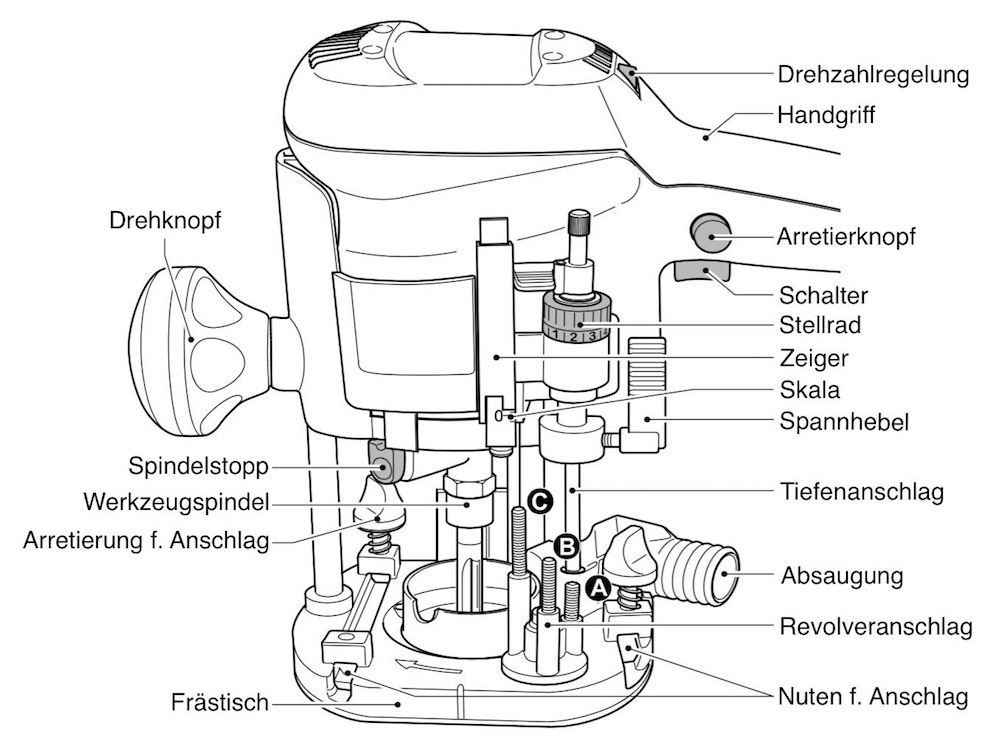
\includegraphics[width=1\textwidth]{img/festool_2.jpg}
	\caption{Übersicht Oberfräse OF 1010 EBQ}
	\label{fig:bilder1}
\end{figure}

\begin{figure}[]
	\centering
	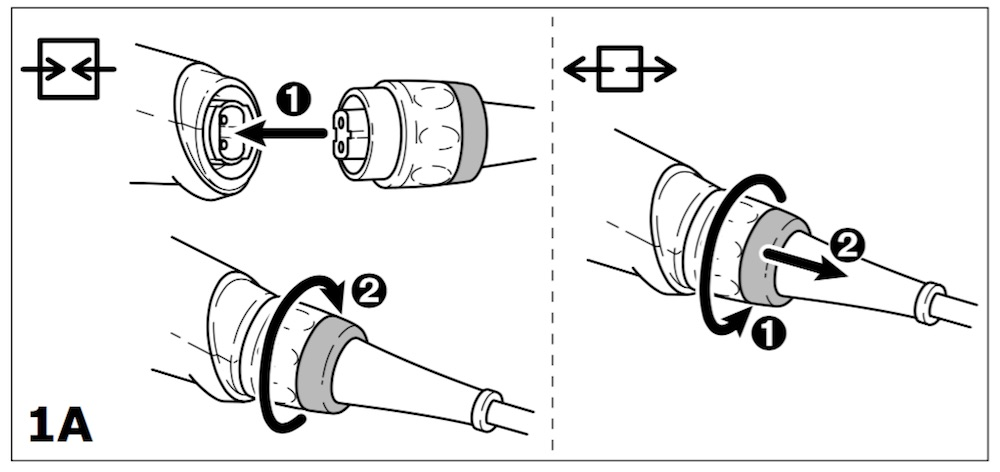
\includegraphics[width=1\textwidth]{img/festool_3.jpg}
	\caption{Montage und Lösen des Netzanschlusses}
	\label{fig:bilder2}
\end{figure}

\begin{figure}[]
	\centering
	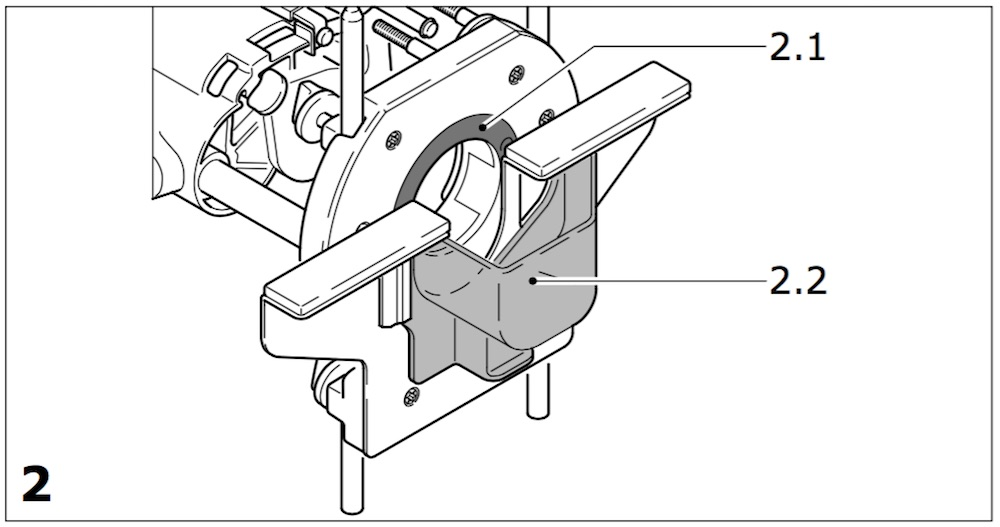
\includegraphics[width=1\textwidth]{img/festool_4.jpg}
	\caption{Zubehör Absaughaube}
	\label{fig:bilder3}
\end{figure}

\begin{figure}[]
	\centering
	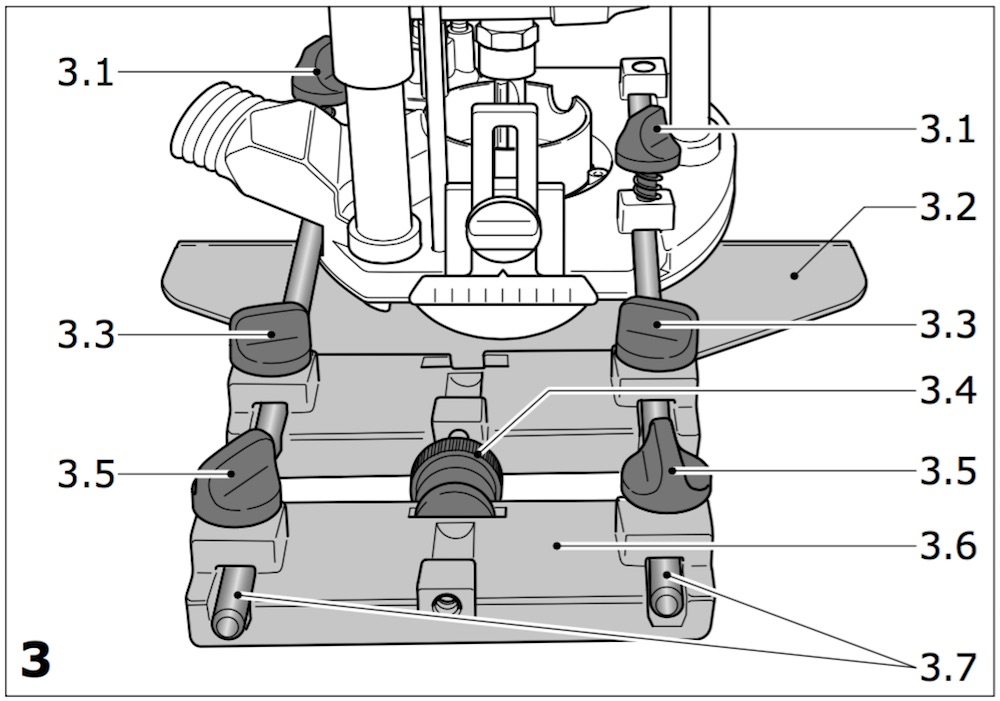
\includegraphics[width=1\textwidth]{img/festool_5.jpg}
	\caption{Seitenanschlag}
	\label{fig:bilder4}
\end{figure}

\begin{figure}[]
	\centering
	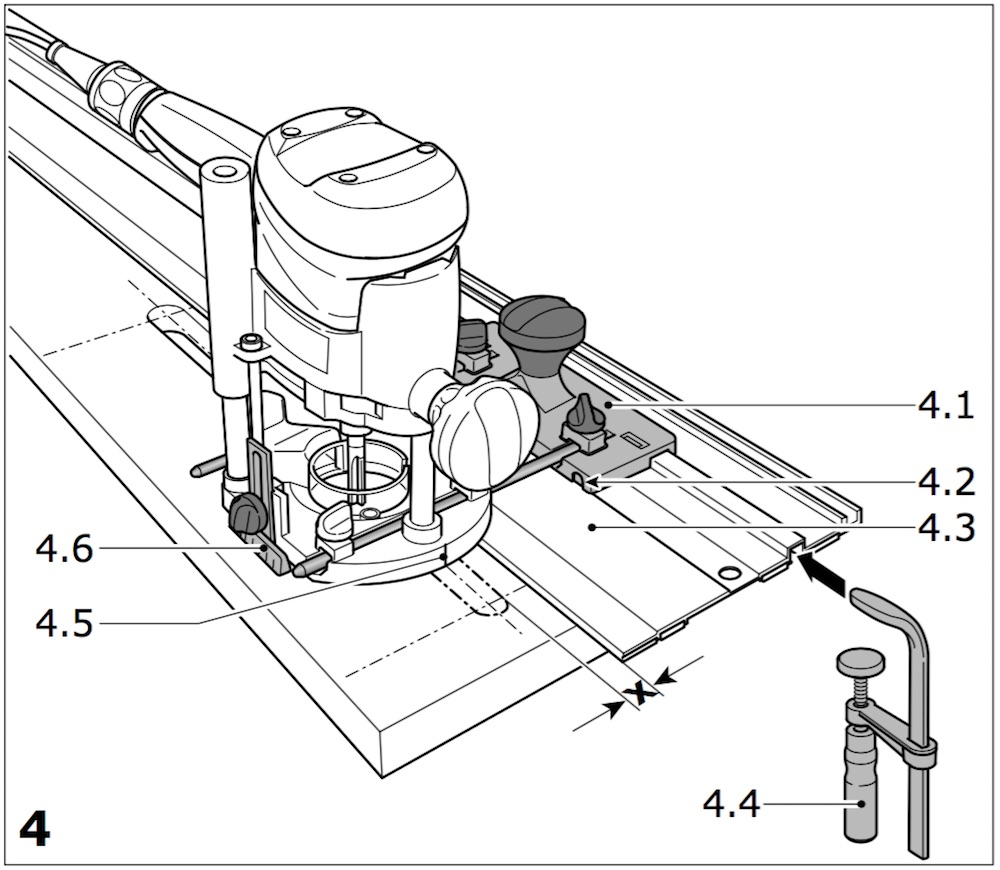
\includegraphics[width=1\textwidth]{img/festool_6.jpg}
	\caption{Führungssystem FS}
	\label{fig:bilder5}
\end{figure}

\begin{figure}[]
	\centering
	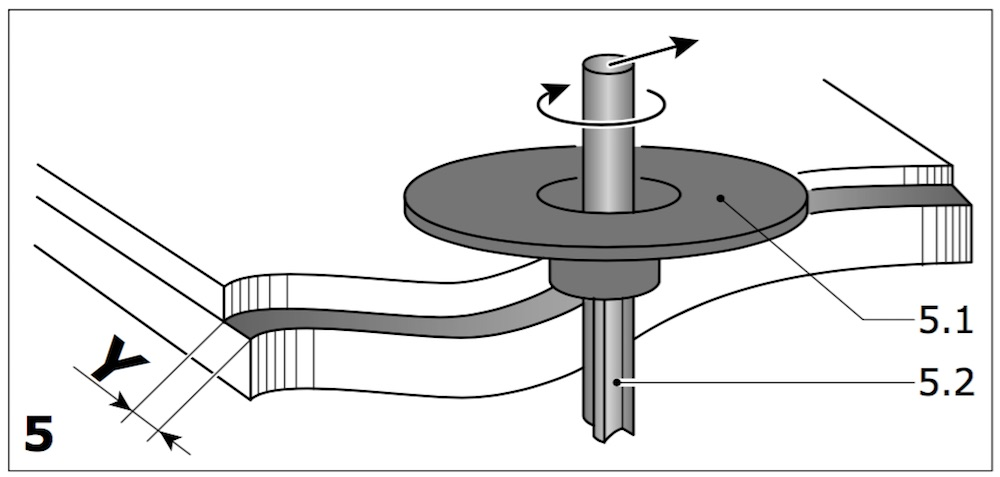
\includegraphics[width=1\textwidth]{img/festool_7.jpg}
	\caption{Zubehör Kopierfräsen: Kopierring}
	\label{fig:bilder6}
\end{figure}

\begin{figure}[]
	\centering
	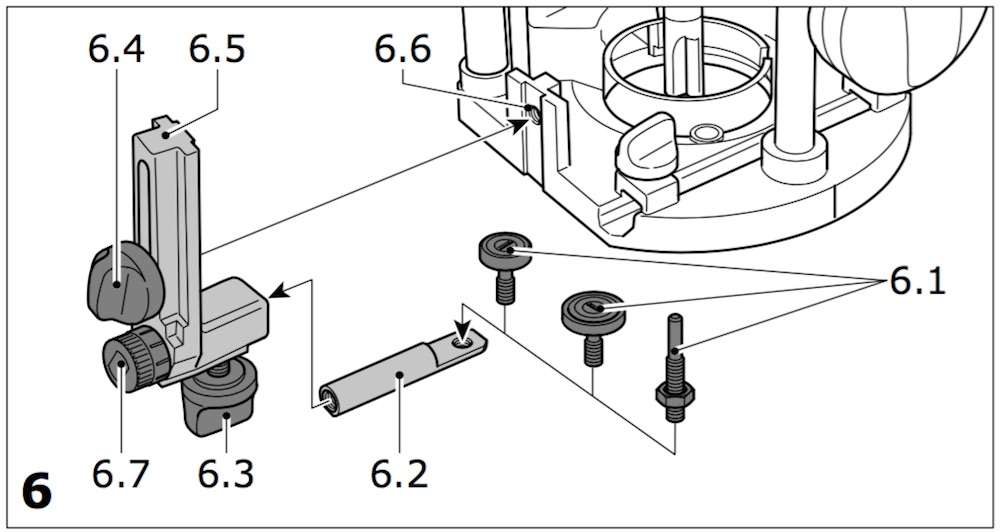
\includegraphics[width=1\textwidth]{img/festool_8.jpg}
	\caption{Zubehör Kopierfräsen: Winkelarm und Rollenhalter}
	\label{fig:bilder7}
\end{figure}

\begin{figure}[]
	\centering
	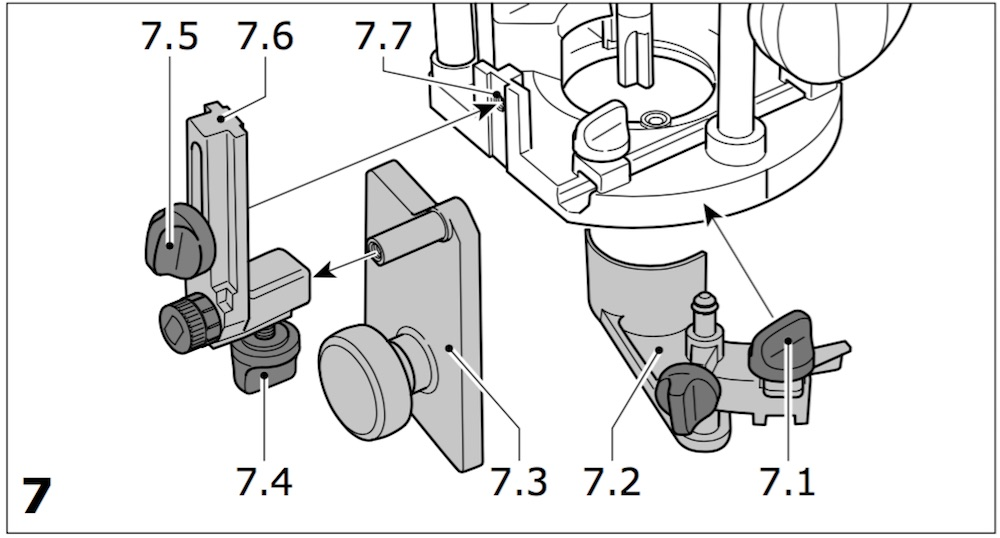
\includegraphics[width=1\textwidth]{img/festool_9.jpg}
	\caption{Zubehör Bündigfräsen}
	\label{fig:bilder8}
\end{figure}

\begin{figure}[]
	\centering
	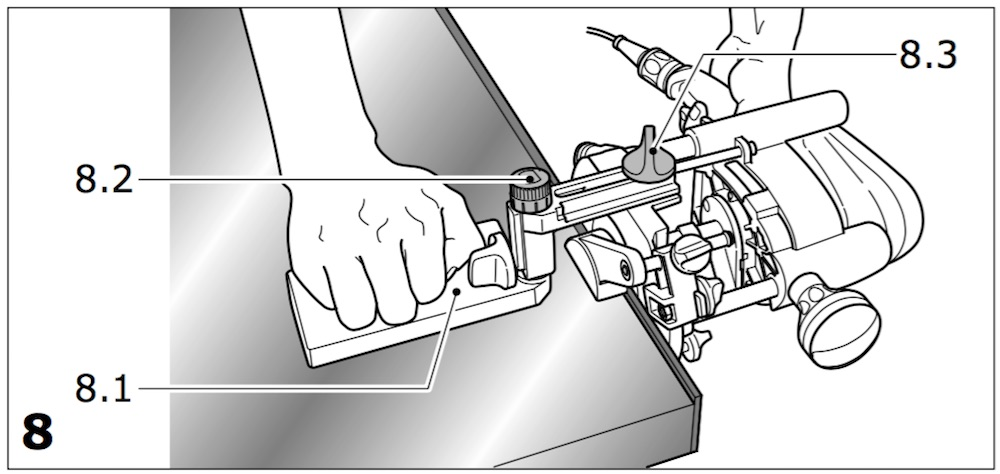
\includegraphics[width=1\textwidth]{img/festool_10.jpg}
	\caption{Zubehör Bündigfräsen}
	\label{fig:bilder9}
\end{figure}

\begin{figure}[]
	\centering
	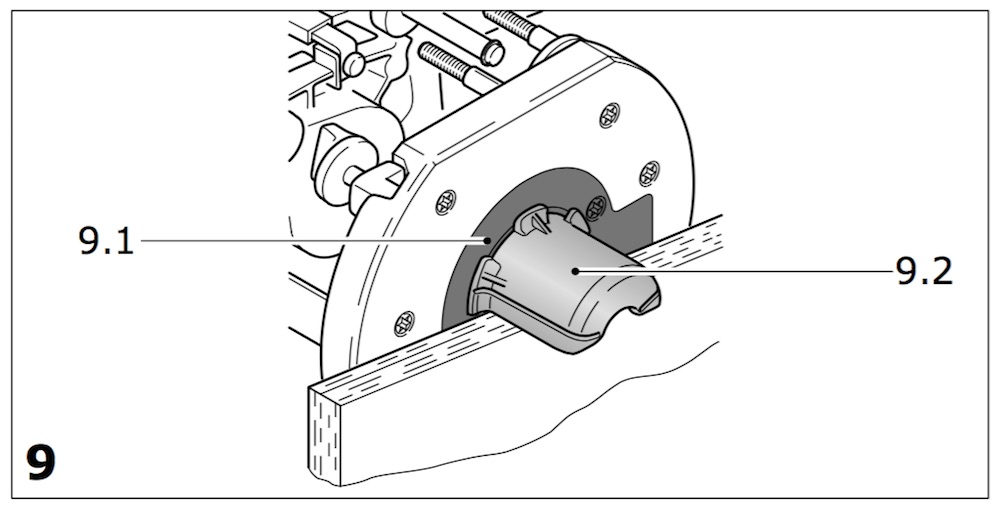
\includegraphics[width=1\textwidth]{img/festool_11.jpg}
	\caption{Zubehör Kantenfräsen: Spanfänger}
	\label{fig:bilder10}
\end{figure}

\newpage
\section{Quellen}
\begin{itemize}
\item Festool \glqq Originalbetriebsanleitung\grqq OF 1010 EBQ unter 
\url{http://www.etracker.de/lnkcnt.php?et=6hsNGE&url=https%3a%2f%2fassets.festool.com%2fmedia%2f468139_007_of1010.zip&lnkname=Bedienungsanleitung+OF+1010+Q%2fEQ%2fEBQ}
\end{itemize}

\end{document}
